\documentclass[12pt,a4paper,notitlepage]{report}
\usepackage[utf8]{inputenc}
\usepackage[english]{babel}

% AMS packages
\usepackage{amsmath}
\usepackage{amsfonts}
\usepackage{amssymb}

\usepackage{eurosym}% euros
\usepackage{listings} % code
% Images
\usepackage{graphicx}
\graphicspath{{images/}}
\usepackage[outdir=images/]{epstopdf}
\usepackage{subfigure}
\DeclareGraphicsExtensions{.pdf,.jpeg,.png,.eps}

\usepackage{todonotes}
\title{LINMA 2470 : Stochastic models}
\author{
  \small
  Malian De Ron
  \and
   \small  
  Florentin Goyens
  \and
  \small
  Quentin Laurent
  \and
  \small
  Harold Taeter
}
\begin{document}
\maketitle
\section*{Model}
We are going to model our bank as a $M/G/2$ queue. Hence the arrival times will follow an exponential law, and the distribution of service time is any distribution where times are positive.
\todo[inline]{Comment traiter le fait qu'un teller est parfois inactif?}
\section*{Parameters estimation}
In order to determine the arrival rate $\lambda$ expressed in $[\frac{1}{s}]$ of the clients in the bank we need to analyse the provided data.


Let $T_{1} \sim Exp(\lambda)$ be the time between the opening of the bank and the arrival of the first client. We then have $T_{2} \sim Exp(\lambda)$ the time between the arrival of the first two clients and so on. The mean of this law is $\frac{1}{\lambda}$. 

 It is easy to convince ourselves that, in the case of our bank, $\lambda$ is a function of time during the day. This allows us to account for rush hours during the day. We first modelized $\lambda$ as a piecewise constant function with three different values during half a day. We will also make a distinction between the morning and the afternoon. We will end up with $6$ values for $\lambda$.
 
 
During a period where it is constant, one can approach $\frac{1}{\lambda}$, the  average time between arrivals as
$$\frac{1}{\lambda}\approx \frac{\sum \text{time between two consecutive arrivals} }{ \text{number of clients arrived}}.$$  

This is similar to using the sample mean estimator for the mean. This is also the maximum likelihood estimator.

If the time period and the number of incomming clients are large enough, we assume reasonable to approach this as
$$\frac{1}{\lambda}\approx \frac{ \text{Time elapsed} }{ \text{number of clients served}}.$$

We have $6$ categories. The value of $\lambda$ for a category is the ration of the clients served during that period over $3600$ seconds, since each range lasts one hour.

\begin{table}
\centering
\begin{tabular}{|c|c|c|c|}
\hline 
$\lambda$ & 9-10h/13-14h & 10-11h/14-15h & 11-12h/15-16h \\ 
\hline 
am & 0.004444 & 0.0063889 & 0.0056944 \\ 
\hline 
pm & 0.0074734 & 0.0084259 & 0.0083333 \\ 
\hline 
\end{tabular}
\caption{Values of the arrival rate $\lambda$.} 
\end{table}

As for the time spend at a desk, we plotted the data of the time spend and tried to guess the distribution. We assumed that this service time is independent of the day of the week and wheter we are in the morning or afternoon. So we gathered all service times available. The histogram can be seen in blue on figure~\ref{lognormal}. We have found that the law follows a lognormal distribution with the following associated parameters for the normal distibution: $\mu= 5.063$ and $\sigma= 0.777$. More precisly, we have shown that the parameters lie respectivly in the $95 \% $ confidence intervals: $\mu \in [ 4.984 , 5.141 ]$ and $\sigma \in [ 0.725 , 0.837]$. Getting back to the mean of the lognormal, she lies in a $1.2$ seconds length interval. This is a small interval compared to the value of the mean: $ 213.7$. We conclude that the choosed lognormal distibution is a good modelization of the service time at a desk.

\begin{figure}[!h]
\centering
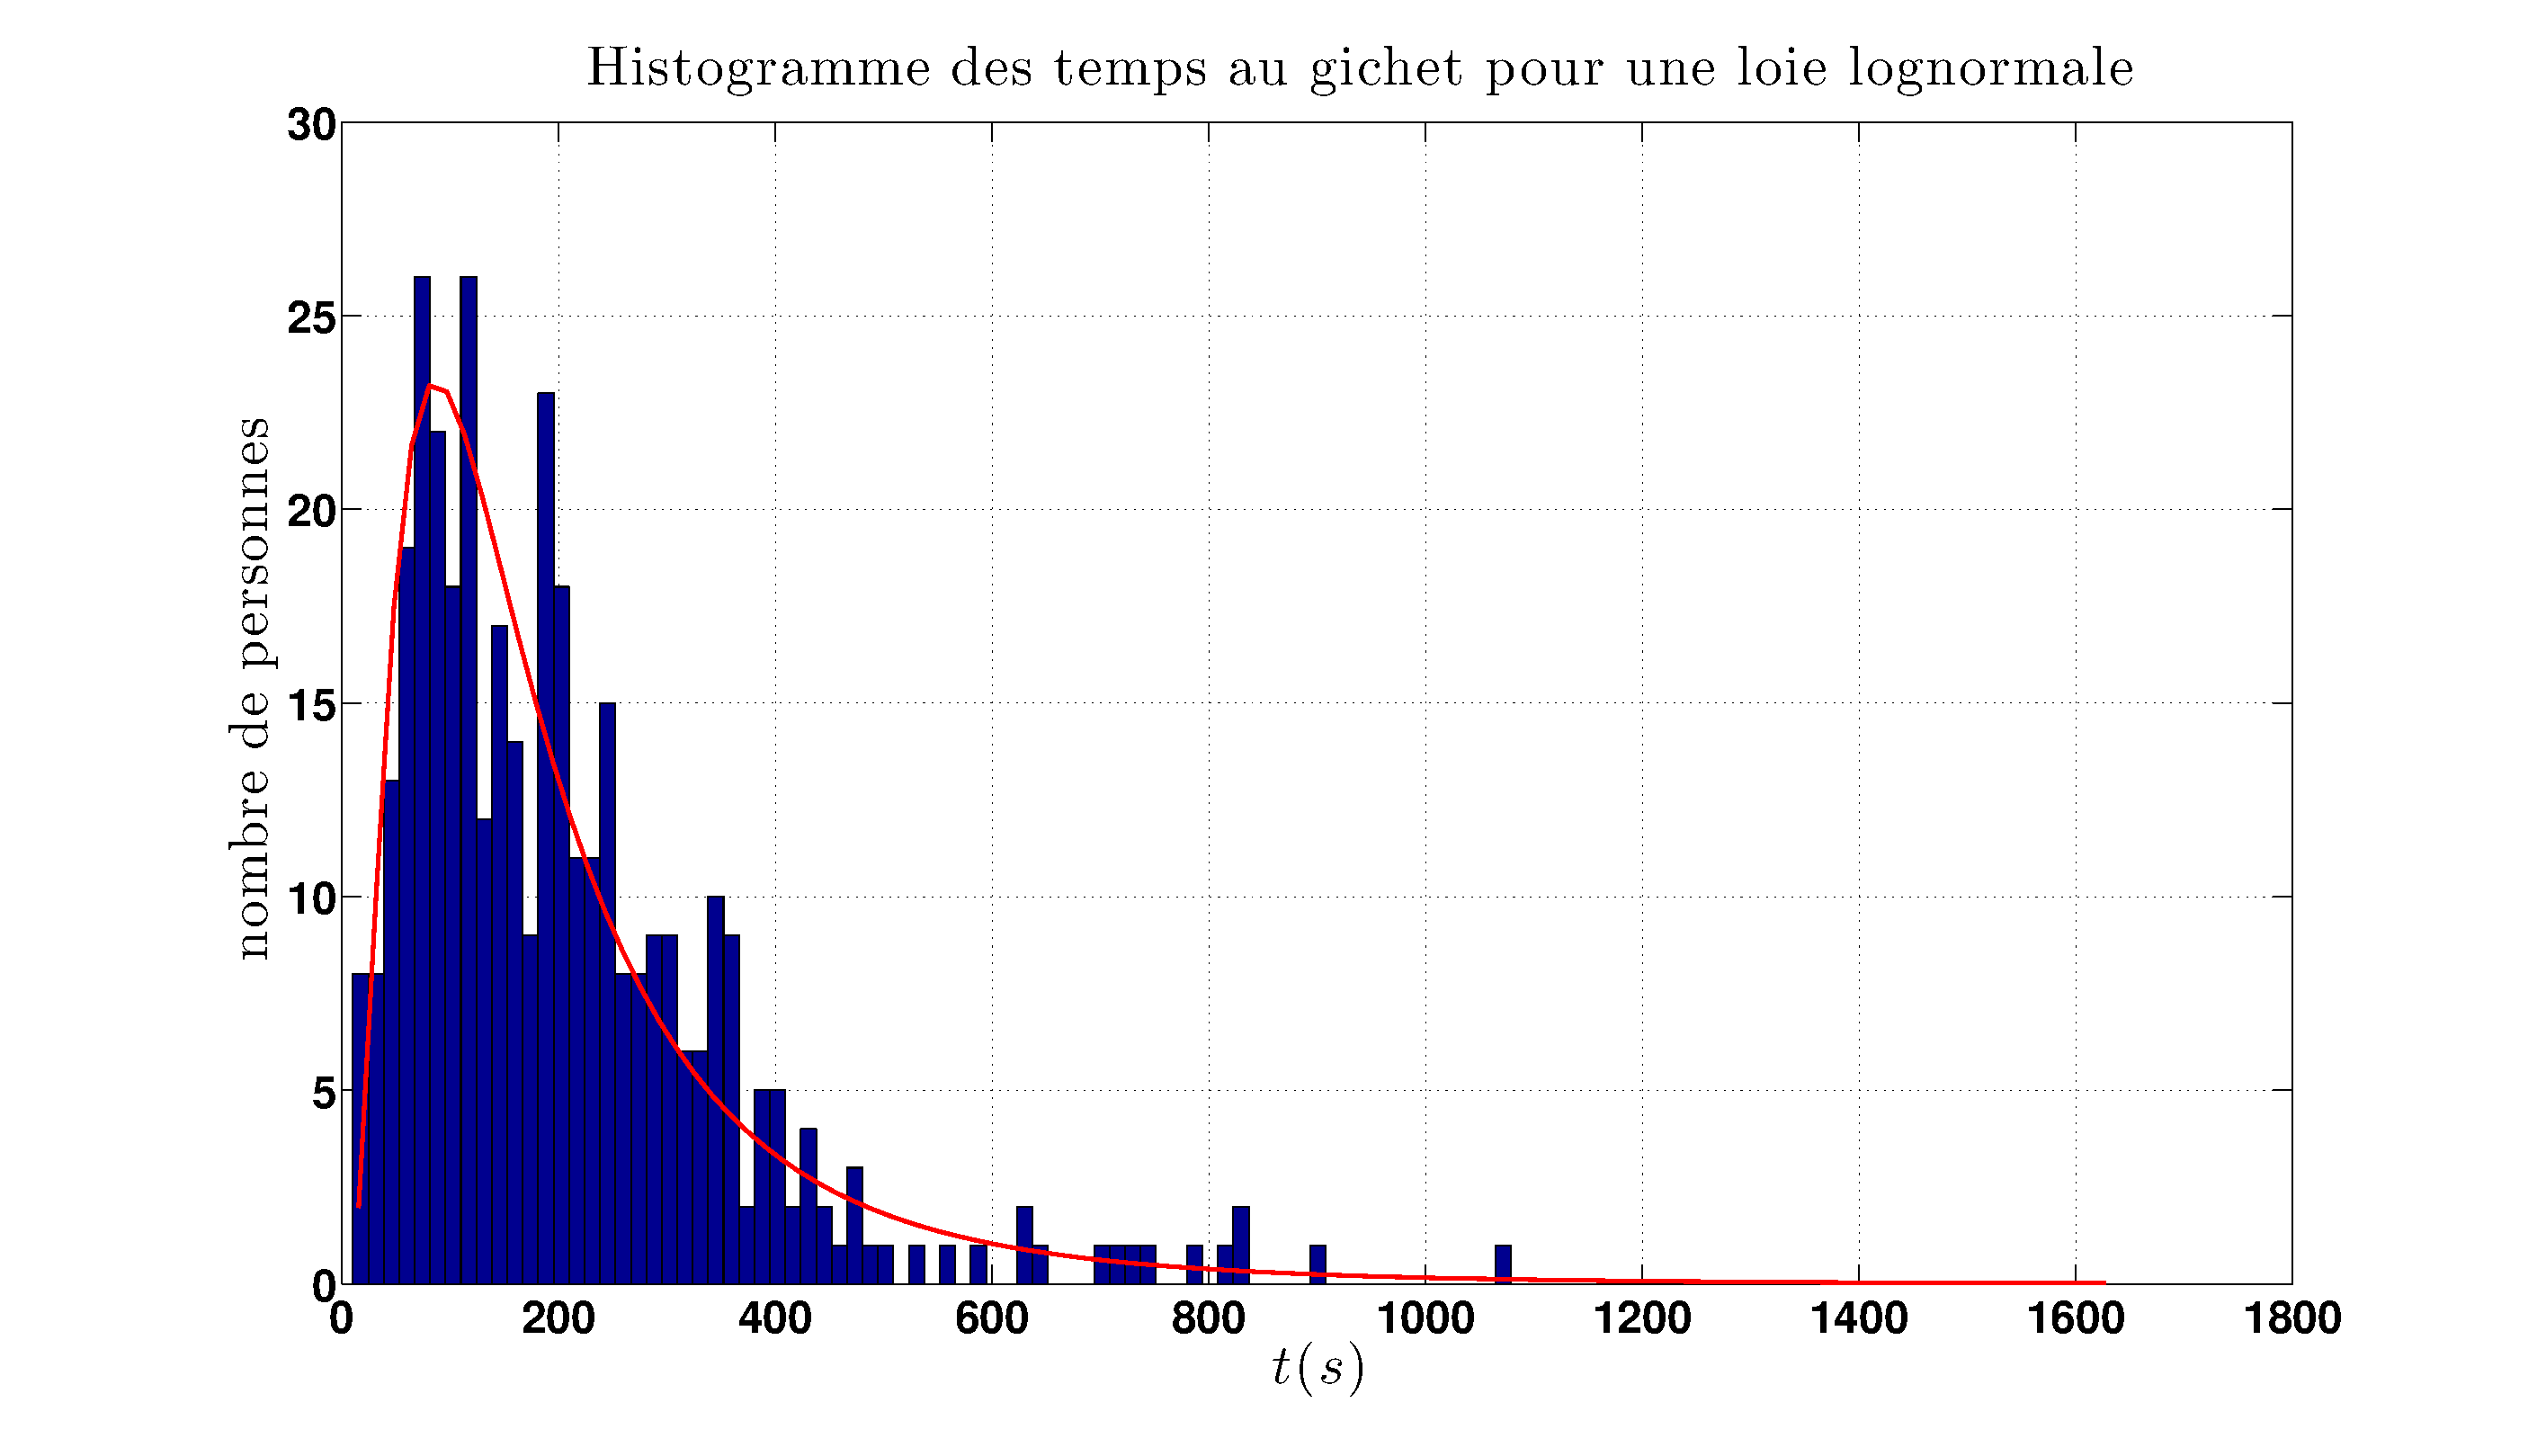
\includegraphics[width = 0.9\textwidth]{./hist_lognormal.eps}
\caption{Lognormal distibution for time spend at a desk.}
\label{lognormal}
\end{figure}


\section*{Anylogic model}

\todo[inline]{Modèle anylogic}

\section*{The merge project}
 Since the clients arriving in the two old branches will sum up and go to the merged branch, we simply add the two Poisson processes, which gives us a new Poisson process with an arrival rate of the clients twice as big as that of the two old branches.

The question that now arises is how many tellers do we really need? Since in each bank a teller is idle at some time, how many of them are needed to make sure that the clients don't wait too much.


In order to estimate the number of tellers necessary for the merged bank, we perform a quasi-steady state approximation of the system. \todo[inline]{explain quasi-steady state approx}

We suppose that the number of tellers is constant throughout the half day considered.
We are trying to minimize a weighted function of the capacity and the total waiting time of the clients.
We consider that the cost of the capacity is proportional to $ \alpha$ (\euro s/customers), and the value of the waiting time of the clients is proportional to $\beta$ (\euro/$s^2$).

Hence, we simply solve the following program :

\begin{eqnarray*}
\min_c & & \alpha c + \beta \int_D A(t)-S(t)\\
\end{eqnarray*}
where $D = \{t | A(t)>=S(t) \}$

So let's now estimate the parameters. Let's say that we pay a teller $S = 75$\euro  a half day, taxes included.
The average processing time is denoted by $\mu$. 
The parameter $\alpha$ is given by $\alpha = \frac{S}{\mu}$
The value of $\beta$ and the other parameters is given in table \ref{table:param}.
\begin{table}
\begin{tabular}{|c|c|c|c|}
\hline 
1/2 day salary(\euro ) & Half day time(s) & $\alpha$(\euro $s$/clients) & $\beta$(\euro/clients$\cdot s$) \\ 
 \hline 
$75$ & $10800$ & $0.433526$ & $3.47222e-07$ \\ 
 \hline 
 
 \end{tabular}
\caption{Parameters\label{table:param}}
\end{table}

Our optimisation problem gives us a value of $ 0.00805561 $ for $c$, which optimizes the capacity in customers per second.\\
It gives us the optimal number of tellers : $N_t = c \mu$
We can see on figure \ref{fig:clients_lun} the approximation of the number of clients arrived in blue and the clients served during the afternoon of monday. We can see that at some point the serving rate of the clients cannot follow the arrival rate of the clients. \\
For the aforementioned parameter values, we get a value of $ 3 $. Of course, it depends on how we value the time of our employers and our customers.
\begin{figure}[h]
\centering
\subfigure[lundi pm]{
\includegraphics[width = 6cm]{half\string_daylundi\string_pm\string_clients\string_served.eps}
}
\subfigure[mardi pm]{
\includegraphics[width = 6cm]{half\string_daymardi\string_pm\string_clients\string_served.eps}
}
\subfigure[mercredi am]{
\includegraphics[width = 6cm]{half\string_daymercredi\string_am\string_clients\string_served.eps}
}
\subfigure[mercredi pm]{
\includegraphics[width = 6cm]{half\string_daymercredi\string_pm\string_clients\string_served.eps}
}
\subfigure[vendredi am]{
\includegraphics[width = 6cm]{half\string_dayvendredi\string_am\string_clients\string_served.eps}
}
\caption{Cumulative amount of clients arrived and served\label{fig:clients_lun}}
\end{figure}



\end{document}
